\documentclass{article}
%Preamble
\usepackage{float}
\usepackage{color}
\usepackage{listings}
\usepackage{longtable}
\usepackage{amsmath,amssymb}
\usepackage{graphics}
\usepackage{graphicx}

\title{AE 625 -Particle Methods in Fluid Flow Simulation \\ Assignment 8: Report \\ SPH Approximation of a function and it's Derivative}
\author{Aditi Taneja}
\date{}

%Preamble
\begin{document}
\pagenumbering{arabic}
\maketitle

$dx =  0.1 $ 
\\
$range  = -1 to 1$
\\
$hdx\_for\_ cubic\_ kernel = 0.7$
\\
$hdx\_ for\_ gaussian\_ kernel = 0.7$


\begin{figure}[H]   \label{figure}
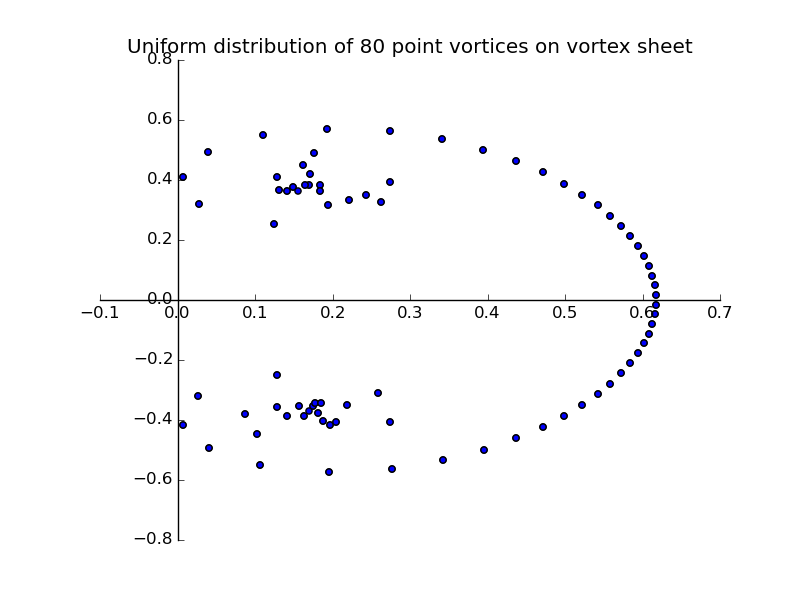
\includegraphics[width=10cm]{one.png}
\caption{Approximation of Sine function with SPH (cubic and Gaussian kernel)}
\label{figure:}
\end{figure}

\begin{figure}[H] \label{figure}
\includegraphics[width=10cm]{error_one.png}
\caption{Variation of Error in approximation of sine function with dx(or number of points)}
\label{figure:}
\end{figure}

\begin{figure}[H] \label{figure}
\includegraphics[width=10cm]{error_two.png}
\caption{Variation of Error in approximation of sine function with hdx(or h)}
\label{figure:}
\end{figure}

\begin{figure}[H] \label{figure}
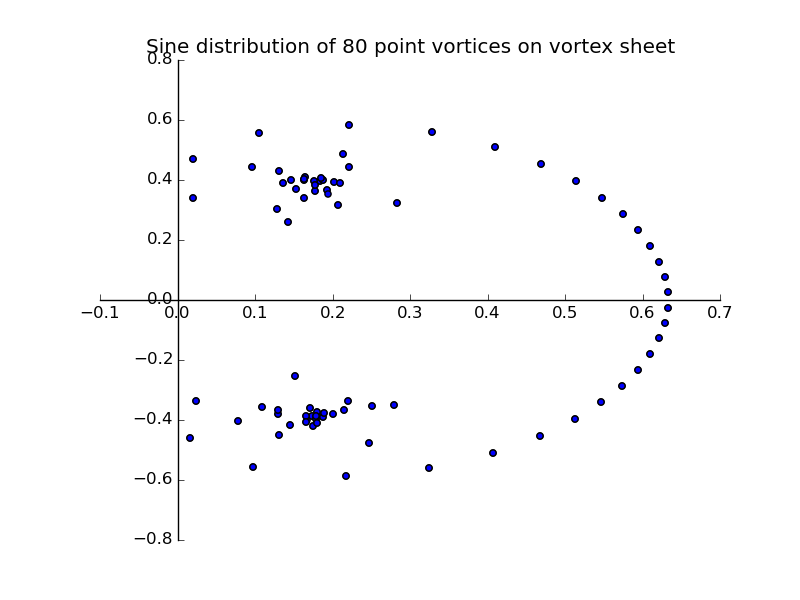
\includegraphics[width=10cm]{two.png}
\caption{Approximation of derivative of Sine function with SPH (cubic and Gaussian kernel)}
\label{figure:}
\end{figure}

\begin{figure}[H] \label{figure}
\includegraphics[width=10cm]{error_three.png}
\caption{Variation of Error in approximation of derivative of sine function with dx(or number of points)}
\label{figure:}
\end{figure}

\begin{figure}[H] \label{figure}
\includegraphics[width=10cm]{error_four.png}
\caption{Variation of Error in approximation of derivative of sine function with hdx(or h)}
\label{figure:}
\end{figure}

Effect of Noise Addition

\begin{figure}[H] \label{figure}
\includegraphics[width=10cm]{error_five.png}
\caption{Variation of Error in approximation of sine function with dx(or number of points) with noise}
\label{figure:}
\end{figure}

\begin{figure}[H] \label{figure}
\includegraphics[width=10cm]{error_six.png}
\caption{Variation of Error in approximation of sine function with hdx(or h) with noise}
\label{figure:}
\end{figure}

\begin{figure}[H] \label{figure}
\includegraphics[width=10cm]{error_seven.png}
\caption{Variation of Error in approximation of derivative of sine function with dx(or number of points) with noise}
\label{figure:}
\end{figure}

\begin{figure}[H] \label{figure}
\includegraphics[width=10cm]{error_eight.png}
\caption{Variation of Error in approximation of derivative of sine function with hdx(or h) with noise}
\label{figure:}
\end{figure}
 
Thus, from the above plots, it can be concluded that as the number of points in the domain are increased or dx is decreased, error decreases (for same hdx) attains a minimum value and then increases.
\\
Also, with increase in hdx error increases.
\\
Noise addition in the particle position can lead to overall increase in error and disrupted plots.
\end{document}
